\documentclass[a4paper,14pt]{extarticle}
\usepackage{../../tex-shared/preamble}

\renewcommand{\mylabnumber}{3}
\renewcommand{\mylabtitle}{Исследование разработки GUI.
Создание sdi-приложений. Обработка событий}
\renewcommand{\mysubject}{Платформа .NET}
\renewcommand{\mylecturer}{Забаштанский А.К.}

\begin{document}
\begin{titlepage}
    
    \thispagestyle{empty}
    
    \begin{center}
        
        Министерство науки и Высшего образования Российской Федерации \\
        Севастопольский государственный университет \\
        Кафедра ИС
        
        \vfill

        Отчет \\
        по лабораторной работе №\mylabnumber \\
        \enquote{\mylabtitle} \\
        по дисциплине \\
        \enquote{\MakeTextUppercase{\mysubject}}

    \end{center}

    \vspace{1cm}

    \noindent\hspace{7.5cm} Выполнил студент группы ИС/б-17-2-о \\
    \null\hspace{7.5cm} Горбенко К. Н. \\
    \null\hspace{7.5cm} Проверил \\
    \null\hspace{7.5cm} \mylecturer

    \vfill

    \begin{center}
        Севастополь \\
        \the\year{}
    \end{center}

\end{titlepage}

\section{Цель работы}
\begin{enumerate}
    \item Изучить принципы разработки графического интерфейса приложений для ОС
    Windows в Visual Studio .Net;
    \item Освоить использование элементов графического интерфейса для
    управления работой приложения;
    \item Освоить принципы построения иерархических меню,
    создания диалоговых окон;
    \item Изучить модель обработки событий в языке C\#.
\end{enumerate}

\section{Задание на работу}
\begin{enumerate}
    \item Создать SDI-приложение (Single Document Interface, однодокументный интерфейс)
    с элементами ввода и отображения полей класса из задания к лабораторной работе 2.
    Для этого используйте различные элементы управления: текстовые поля, списки,
    независимые и радиокнопки, а также панели и менеджеры компоновки.
    \item Ввод новых данных осуществлять через дополнительную диалоговую форму.
    \item При изменении данных запрашивать подтверждение через окно диалога.
    В случае неполных данных сообщать об ошибке.
    \item Объекты сохранять в коллекции.
    \item Реализовать просмотр всей коллекции объектов через список.
    Для редактирования выбранного объекта создать дополнительную форму
    модального диалога.
    \item Добавить на форму меню, позволяющее работать с пунктами:
    добавить, просмотреть, удалить, редактировать, справка.
    \item Дублировать основные операции панелью инструментов.
\end{enumerate}

Для варианта № 3 задана следующая схема данных:
\textbf{ПЕЧАТНОЕ ИЗДАНИЕ: название, ФИО автора, стоимость}
\section{Ход работы}
Создадим \code{WPF} проект на \code{.NET Core 3.0}, создадим главную
страницу приложения. Точкой входа приложения является окно \code{App.xaml}.
Разработку будем осуществлять с помощью паттерна MVVM, поддерживаемого WPF.
Зададим в нем ссылку на главную страницу:
\begin{lstlisting}
<Application x:Class="PrintedEditionSdiApp.App"
             xmlns="http://schemas.microsoft.com/winfx/2006/xaml/presentation"
             xmlns:x="http://schemas.microsoft.com/winfx/2006/xaml"
             StartupUri="Views/MainWindow.xaml">
</Application>
\end{lstlisting}

\subsection{Главная страница}
Создадим главную страницу \code{MainWindow.xaml}. В ней зададим представление
главной страницы - \code{PrintedEditionControl}, размеры окна. Свойство
\code{ResizeMode} в данном случае используется для запрета возможности
изменения размеров окна.
\begin{lstlisting}
<Window x:Class="PrintedEditionSdiApp.Views.MainWindow"
    ...
    xmlns:views="clr-namespace:PrintedEditionSdiApp.Views"
    Title="PrintedEditionMainWindow"
    ResizeMode="NoResize"
    Width="400" Height="500">

<views:PrintedEditionControl/>
</Window>
\end{lstlisting}

Опишем представление \code{PrintedEditionControl}. Оно включает \code{StackPanel}. \code{StackPanel},
в свою очередь, включает \code{ListView} со списком доступных печатных изданий. Под списком находится
три текстовых поля, предоставляющих информацию о выбранном печатном издании. Поля заблокированы с помощью
свойства \code{IsEnabled} т.к. редактирование должно осуществляться в отдельном окне. Список изданий
привязан к коллекции вью модели, соответствующей этой странице. Выбранное издание привязано к свойству
вью модели. Все привязки осуществляются с помощью биндингов MVVM.
\begin{lstlisting}
<Page x:Class="PrintedEditionSdiApp.Views.PrintedEditionControl"
      ...
      mc:Ignorable="d"
      Title="PrintedEditionMainWindow"
      d:DataContext="{d:DesignInstance viewModels:PrintedEditionViewModel}">
    
    <StackPanel>
        <StackPanel>
            <Label HorizontalAlignment="Center">Printed Editions</Label>
            <ListView ItemsSource="{Binding PrintedEditions}" SelectedItem="{Binding SelectedPrintedEdition}"
                      ScrollViewer.VerticalScrollBarVisibility="Visible"
                      Height="250" Margin="5">
                <ListView.Resources>
                    <Style TargetType="ListViewItem">
                        <Style.Triggers>
                            <Trigger Property="IsKeyboardFocusWithin" Value="True">
                                <Setter Property="IsSelected" Value="True"/>
                            </Trigger>
                        </Style.Triggers>
                    </Style>
                </ListView.Resources>
                <ListView.ItemTemplate>
                    <DataTemplate>
                        <Grid>
                            <Grid.ColumnDefinitions>
                                <ColumnDefinition Width="240"/>
                                <ColumnDefinition Width="50" />
                                <ColumnDefinition Width="50" />
                            </Grid.ColumnDefinitions>
                            <StackPanel Grid.Column="0" Margin="5">
                                <TextBlock Text="{Binding Name}" />
                                <TextBlock Text="{Binding Author}" />
                                <TextBlock Text="{Binding Price}" />
                            </StackPanel>
                            <Button Grid.Column="1"
                                    Click="EditPrintedEditionButtonClick"
                                    Margin="5" Content="Edit"/>
                            <Button Grid.Column="2"
                                    Command="{Binding Path=DataContext.DeleteCommand,
                                              RelativeSource={RelativeSource FindAncestor,
                                              AncestorType={x:Type Page}}}"
                                    Margin="5" Content="Delete"/>
                        </Grid>
                    </DataTemplate>
                </ListView.ItemTemplate>
            </ListView>
            <Button Click="AddPrintedEditionButtonClick" Margin="5">Add</Button>
        </StackPanel>
        
        <StackPanel IsEnabled="False" DataContext="{Binding SelectedPrintedEdition}" Margin="5">
            <Label HorizontalAlignment="Center">Selected Edition</Label>
            <TextBlock Text="Name" />
            <TextBox Text="{Binding Name, UpdateSourceTrigger=PropertyChanged}" />
            <TextBlock Text="Author" />
            <TextBox Text="{Binding Author, UpdateSourceTrigger=PropertyChanged}" />
            <TextBlock Text="Price" />
            <TextBox Text="{Binding Price, UpdateSourceTrigger=PropertyChanged}" />
        </StackPanel>
    </StackPanel>
</Page>
\end{lstlisting}

Вид главной страницы:
\begin{figure}[H]
    \centering
    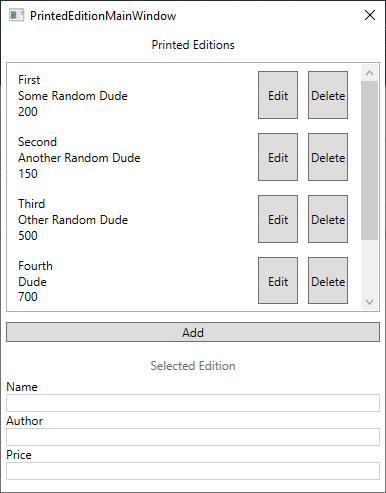
\includegraphics[width=.6\linewidth]{PrintedEditionControl}
    \caption{Вид главного окна приложения}
    \label{fig:printed-edition-control}
\end{figure}

Создадим соответствующую этой странице вью модель. Она содержит коллекцию \code{PrintedEditions},
свойство \code{SelectedPrintedEdition}, методы для добавления, изменения и удаления печатных изданий.
Любое изменение любого свойства вью модели приведет к триггеру события \code{PropertyChanged}.
Это событие опевестит представление о том, что какое-то свойство изменилось, что приведет к
обновлению представления. Методы редактирования и добавления печатного издания используется другими
вью моделями.
\begin{lstlisting}
public class PrintedEditionViewModel : INotifyPropertyChanged
{
    private static PrintedEditionViewModel instance;
    private PrintedEdition selectedPrintedEdition;
    private ICommand deleteCommand;

    public event PropertyChangedEventHandler PropertyChanged;
    public ObservableCollection<PrintedEdition> PrintedEditions { get; set; }

    public PrintedEdition SelectedPrintedEdition
    {
        get => selectedPrintedEdition;
        set
        {
            selectedPrintedEdition = value;
            OnPropertyChanged(nameof(SelectedPrintedEdition));
        }
    }

    public ICommand DeleteCommand =>
        deleteCommand ??= new RelayCommand(
            obj => RemovePrintedEdition(selectedPrintedEdition),
            obj => true);

    [NotifyPropertyChangedInvocator]
    protected virtual void OnPropertyChanged([CallerMemberName] string propertyName = null)
    {
        PropertyChanged?.Invoke(this, new PropertyChangedEventArgs(propertyName));
    }

    public static PrintedEditionViewModel GetInstance()
    {
        return instance ??= new PrintedEditionViewModel();
    }

    private PrintedEditionViewModel()
    {
        PrintedEditions = new ObservableCollection<PrintedEdition>
        {
            new PrintedEdition { Id = 1, Name = "First", Author = "Some Random Dude", Price = 200},
            new PrintedEdition { Id = 2, Name = "Second", Author = "Another Random Dude", Price = 150},
            new PrintedEdition { Id = 3, Name = "Third", Author = "Other Random Dude", Price = 500},
            new PrintedEdition { Id = 4, Name = "Fourth", Author = "Dude", Price = 700}
        };
    }

    public void AddPrintedEdition(PrintedEdition printedEdition)
    {
        if (printedEdition == null)
        {
            throw new ArgumentNullException(nameof(printedEdition));
        }

        if (printedEdition.Id == 0)
        {
            printedEdition.Id = GetUniqueId();
        }
        PrintedEditions.Add(printedEdition);
    }

    public void RemovePrintedEdition(PrintedEdition printedEdition)
    {
        if (printedEdition == null)
        {
            throw new ArgumentNullException(nameof(printedEdition));
        }

        if (PrintedEditions.Contains(printedEdition))
        {
            PrintedEditions.Remove(printedEdition);
        }
    }

    public void ReplacePrintedEdition(PrintedEdition printedEdition)
    {
        if (printedEdition == null)
        {
            throw new ArgumentNullException(nameof(printedEdition));
        }

        var oldPrintedEdition = PrintedEditions.FirstOrDefault(x => x.Id == printedEdition.Id);
        if (oldPrintedEdition != null)
        {
            oldPrintedEdition.Name = printedEdition.Name;
            oldPrintedEdition.Author = printedEdition.Author;
            oldPrintedEdition.Price = printedEdition.Price;
        }
    }

    private int GetUniqueId()
    {
        var generator = new Random();
        var uniqueId = 0;

        while (PrintedEditions.FirstOrDefault(x => x.Id == uniqueId) != null)
        {
            uniqueId = generator.Next();
        }

        return uniqueId;
    }
}
\end{lstlisting}

\subsection{Окно создания}
Создадим окно создания печатного издания и его вью модель:
\begin{lstlisting}
<Window x:Class="PrintedEditionSdiApp.Views.AddPrintedEditionWindow"
    ...
    xmlns:viewModels="clr-namespace:PrintedEditionSdiApp.ViewModels"
    Title="PrintedEditionMainWindow"
    Width="400" Height="210"
    d:DataContext="{d:DesignInstance viewModels:AddPrintedEditionViewModel}">

    <StackPanel>
        <StackPanel DataContext="{Binding PrintedEditionToAdd}" Margin="5">
            <Label HorizontalAlignment="Center">Enter printed edition details</Label>
            <TextBlock Text="Name" />
            <TextBox Text="{Binding Name}" />
            <TextBlock Text="Author" />
            <TextBox Text="{Binding Author}" />
            <TextBlock Text="Price" />
            <TextBox Text="{Binding Price}" />
        </StackPanel>
        <Button Command="{Binding AddPrintedEditionCommand}" Click="AddButtonClick" Margin="5" Content="Add">
        </Button>
    </StackPanel>
</Window>
\end{lstlisting}

\begin{lstlisting}
public class AddPrintedEditionViewModel : INotifyPropertyChanged
{
    private PrintedEdition printedEditionToAdd;
    private readonly PrintedEditionViewModel printedEditionViewModel;
    private ICommand addPrintedEditionCommand;

    public event PropertyChangedEventHandler PropertyChanged;
    public PrintedEdition PrintedEditionToAdd
    {
        get => printedEditionToAdd;
        set
        {
            printedEditionToAdd = value;
            OnPropertyChanged(nameof(PrintedEditionToAdd));
        }
    }

    public ICommand AddPrintedEditionCommand =>
        addPrintedEditionCommand ??= 
            new RelayCommand(
                obj => AddPrintedEdition(printedEditionToAdd),
                obj => true);

    [NotifyPropertyChangedInvocator]
    protected virtual void OnPropertyChanged([CallerMemberName] string propertyName = null)
    {
        PropertyChanged?.Invoke(this, new PropertyChangedEventArgs(propertyName));
    }

    public AddPrintedEditionViewModel()
    {
        printedEditionToAdd = new PrintedEdition();
        printedEditionViewModel = PrintedEditionViewModel.GetInstance();
    }

    private void AddPrintedEdition(PrintedEdition printedEdition)
    {
        if (printedEdition == null)
        {
            throw new ArgumentNullException(nameof(printedEdition));
        }

        printedEditionViewModel.AddPrintedEdition(printedEdition);
    }
}
\end{lstlisting}

Вид диалога добавления печатного издания:
\begin{figure}[H]
    \centering
    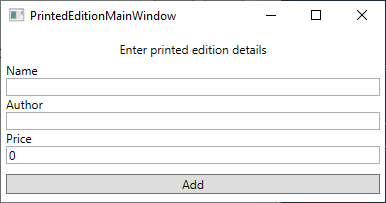
\includegraphics[width=.6\linewidth]{Add}
    \caption{Вид диалога добавления печатного издания}
    \label{fig:add}
\end{figure}

\subsection{Диалог редактирования}
Создадим диалог редактирования и его вью модель:
\begin{lstlisting}
<Window x:Class="PrintedEditionSdiApp.Views.EditPrintedEditionWindow"
    ...
    xmlns:viewModels="clr-namespace:PrintedEditionSdiApp.ViewModels"
    Title="PrintedEditionEditFormWindow" Width="400" Height="210"
    d:DataContext="{d:DesignInstance viewModels:EditPrintedEditionViewModel}">
    
    <StackPanel>
        <StackPanel DataContext="{Binding PrintedEditionToEdit}" Margin="5">
            <Label HorizontalAlignment="Center">Enter printed edition details</Label>
            <TextBlock Text="Name" />
            <TextBox Text="{Binding Name}" />
            <TextBlock Text="Author" />
            <TextBox Text="{Binding Author}" />
            <TextBlock Text="Price" />
            <TextBox Text="{Binding Price}" />
        </StackPanel>
        <Button Command="{Binding EditPrintedEdition}" Click="EditButtonClick" Margin="5">Edit</Button>
    </StackPanel>
</Window>
\end{lstlisting}
    
\begin{lstlisting}
public class EditPrintedEditionViewModel : INotifyPropertyChanged
{
    private PrintedEdition printedEditionToEdit;
    private readonly PrintedEditionViewModel printedEditionViewModel;
    private ICommand editPrintedEdition;

    public event PropertyChangedEventHandler PropertyChanged;

    public PrintedEdition PrintedEditionToEdit
    {
        get => printedEditionToEdit;
        set
        {
            printedEditionToEdit = value;
            OnPropertyChanged(nameof(PrintedEditionToEdit));
        }
    }

    public ICommand EditPrintedEdition =>
        editPrintedEdition ??= new RelayCommand(
            obj => ReplacePrintedEdition(printedEditionToEdit), 
            obj => true);

    public EditPrintedEditionViewModel(PrintedEdition printedEdition)
    {
        printedEditionToEdit = printedEdition ?? throw new ArgumentNullException(nameof(printedEdition));
        printedEditionViewModel = PrintedEditionViewModel.GetInstance();
    }

    [NotifyPropertyChangedInvocator]
    protected virtual void OnPropertyChanged([CallerMemberName] string propertyName = null)
    {
        PropertyChanged?.Invoke(this, new PropertyChangedEventArgs(propertyName));
    }

    private void ReplacePrintedEdition(PrintedEdition printedEdition)
    {
        if (printedEdition == null)
        {
            throw new ArgumentNullException(nameof(printedEdition));
        }
        
        printedEditionViewModel.ReplacePrintedEdition(printedEdition);
    }
}
\end{lstlisting}

Вид диалога редактирования печатного издания:
\begin{figure}[H]
    \centering
    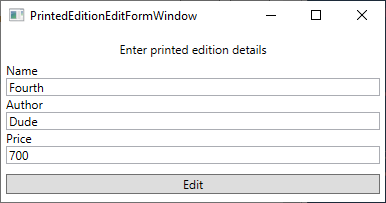
\includegraphics[width=.6\linewidth]{Edit}
    \caption{Вид диалога редактирования печатного издания}
    \label{fig:edit}
\end{figure}

\section*{Выводы}
В ходе лабораторной работы были изучены основы создания десктопных приложений под Windows
на платформе .NET. Для создания приложений на WPF используется паттерн MVVM, основанный на
разделении представления приложения от его логики. Реализовывается паттерн за счет событий
платформы .NET.

Для создания представления используются классы разметки с расширением \code{xaml}. Каждый класс
может содержать только один элемент. Для того, чтобы поместить на странице несколько элементов,
их необходимо объединить в один с помощью высокоуровневых контролов: \code{StackPanel}, \code{Grid},
\code{WrapPanel} и других.
\end{document}